\documentclass{report}
\usepackage[utf8]{inputenc}
\usepackage[T1]{fontenc}
\usepackage[french]{babel}% traduction des noms chapitre, section, etc.
\frenchbsetup{StandardLists=true} % on garde les belles puces

\usepackage[top=2cm, bottom=2cm, left=2.5cm, right=2.5cm]{geometry}
\usepackage{amsmath, amssymb, mathrsfs, stmaryrd, amsthm} % pr les maths
\usepackage{listings} % pour code source
\usepackage{graphicx,caption, subcaption} % pr image
\usepackage{multicol}
\usepackage[hidelinks]{hyperref}  % sommaire cliquable
\usepackage{url}
\usepackage{listings} % pour code source
\usepackage{color}
\definecolor{deepblue}{rgb}{0,0,0.5}
\definecolor{deepred}{rgb}{0.6,0,0}
\definecolor{deepgreen}{rgb}{0,0.5,0}
\DeclareFixedFont{\ttb}{T1}{txtt}{bx}{n}{12} % for bold
\DeclareFixedFont{\ttm}{T1}{txtt}{m}{n}{12}  % for normal
\lstset{
breaklines=true,
numbers=left,
language=Python,
basicstyle=\ttm,
otherkeywords={self},             % Add keywords here
keywordstyle=\ttb\color{deepblue},
emph={MyClass,__init__},          % Custom highlighting
emphstyle=\ttb\color{deepred},    % Custom highlighting style
stringstyle=\color{deepgreen},
frame=tb,                         % Any extra options here
showstringspaces=false            % 
}



\newtheorem*{lemma}{Lemme} % La petite étoile enlève la numérotation, mais nécessite le package amsthm
\newtheorem{theorem}{Théorème}[chapter]
\newtheorem{property}[theorem]{Proposition}    
\newtheorem{definition}{Définition}[chapter] % Le [chapter] peut par exemple êtreremplacé par [section], il permet de numéroter les éléments par rapport aux numéros de chapitre
\newtheorem{corollary}{Corollaire}[theorem]
\newtheorem{conjecture}{Conjecture}


\renewcommand\qedsymbol{$\blacksquare$}  % change le carré de fin de démo



\newcommand{\parite}[1]{\ensuremath{\text{Paritée}(#1)}}
\newcommand{\parcours}[2]{\ensuremath{\text{Parcours}(#1 \times #2)}}
\newcommand{\trajet}[6]{\ensuremath{\text{Trajet}(#1 \times #2; (#3, #4); (#5; #6))}}
\newcommand{\pa}[2]{\ensuremath{\text{P}_A(#1 \times #2)}}
\newcommand{\pb}[2]{\ensuremath{\text{P}_B(#1 \times #2)}}
\newcommand{\po}[2]{\ensuremath{\text{P}_O(#1 \times #2)}}
\newcommand{\Pm}[1]{\ensuremath{\text{P}_M(#1)}}
\newcommand{\pythonlogo}{\includegraphics[width=1em , height=2ex]{python128.png}}

\newcommand{\poids}[1]{\ensuremath{\text{Poids}(#1)}}
\newcommand{\recu}[1]{\ensuremath{\mathcal{R}\text{ec}(#1)}}
\newcommand{\nrecu}[1]{\ensuremath{\text{SNR}(#1)}}
\newcommand{\conf}[1]{\ensuremath{\text{S}(#1)}}
\newcommand{\confull}[1]{\ensuremath{\delta_{#1}}}
\newcommand{\poidsmin}[1]{\ensuremath{\mu_{#1}}}
\newcommand{\stab}[1]{\ensuremath{\widehat{#1}}}
\newcommand{\avalanche}[1]{\ensuremath{\text{Avalanche}(#1)}}
\newcommand{\diag}[1]{\ensuremath{\text{Diag}(#1)}}
\newcommand{\plus}{\ensuremath{\oplus}}
\newcommand{\card}[1]{\ensuremath{|#1|}}

\title{Automates de tas de sable}
\author{Théo \textsc{Rudkiewicz}}

\begin{document}
\maketitle
\newpage
\tableofcontents

\chapter{Introduction}

Les automates cellulaires ont été développés par Von Neuman dans les années 1940. Un automateest régi par quelques règles locales simples qui créent des comportements complexes à plus grandeéchelle. Un automate peut ainsi représenter un phénomène physique : une fois les règlesmicroscopiques décrites, on peut en observer les effets macroscopiques. 

Le déplacement d’amas de sable peut s’étudier avec un automate cellulaire %\cite{DRPWPC}. 
J’ai choisi le modèledu tas de sable abélien. Cet automate créé en 1980 par Bak, Tang et Wisenfeld \cite{thTang} est constituéd’une grille quadratique sur laquelle des grains de sable sont placés et s’éboulent sur les casesadjacentes. On peut alors définir un processus markovien par l’ajout successif de grains placésaléatoirement suivi d’une stabilisation par éboulement. On distingue alors les configurationstransitoires apparaissant un nombre fini de fois et celles récurrentes apparaissant un nombre infinide fois. Une question qui se pose alors est la probabilité d’apparition d’une configuration récurrente.On démontre que toutes les configurations récurrentes sont équiprobables \cite{thDhar}. La propriétéfondamentale du modèle est l’apparition spontanée de configurations dites critiques. A partir d’unetelle configuration il est possible d’observer de grandes ou de petites avalanches. Par ailleurs, onretrouve une loi puissance pour la distribution des amplitudes des avalanches. La loi puissance se
retrouve aussi pour la magnitude des séismes et d’autres phénomènes naturels. Cependant, lecoefficient de cette loi pour le tas de sable reste inconnu \cite{thPoly}. 

Ce modèle est ensuite généralisé à n’importe quel graphe. En munissant l’ensemble desconfigurations récurrentes d’une loi qui combine l’addition sommet à sommet du nombre de grainssuivie de la stabilisation, on obtient un groupe abélien, d’où le nom du modèle \cite{thDhar}. En considérantune configuration comme un vecteur de $Z^n$, on peut dire que $Z^n$ quotienté par le sous-groupeengendré par les opérateurs d’éboulement est un groupe dont les représentants canoniques sont lesconfigurations récurrentes. Deepak Dahr fournit de plus un algorithme appelé algorithme thermiquepermettant de donner la configuration équivalente à une configuration donnée. De cet algorithmedérive également un critère, appelé critère de Dahr, permettant de discriminer les configurations récurrentes. De plus, on obtient facilement le neutre car celui-ci équivaut à la configuration nulle. Enfin, on peut aussi chercher l’ordre (le cardinal) du groupe. Pour cela, Dahr établit une bijectionentre les arbres couvrants et les configurations récurrentes. Grâce au théorème de Kirchhoff sur lesgraphes, l’ordre s’en déduit.

Enfin, pour le graphe original rectangulaire dans $Z^2$, on peut voir apparaître des fractales. Parexemple, la forme du neutre est étudiée dans la thèse de Dartois \cite{thPoly}. Le résultat de l’éboulementd’un grand nombre de grains (n) depuis une unique case forme un cercle de rayon racine de n \cite{geoid} .Cependant, il n’existe pas pour le moment d’explication à l’apparition d’auto-similarités. 

Finalement, il existe une recherche active autour du modèle du tas de sable abélien \cite{thBordeaux}. D’une part,nombre de propriétés géométriques sur la grille $Z^2$ sont non démontrées. D’autre part desextensions du modèle sont proposées comme le modèle de flèche hauteur \cite{thPoly} ou le tas de sable divisible \cite{divisible}.

\chapter{Présentation du modèle}
\section{Forme et configurations}

La forme d'un tas de sable est donné par un graphe connexe G=(S, A) (dans notre cas non orienté). On numérote les sommets de 0 à $n$. Dans toute la suite, on a $n := \card{S} - 1$.
Un sommet est distingué et appelé puits, il est numéroté 0 (avec $S^*$ les sommets sans le puits). On note $\Delta$ le laplacien du graphe, $\Delta^q$ le laplacien réduit où l'on a supprimé la ligne et la colonne associées au puits, $\diag{\Delta^q}$ la diagonale de $\Delta^q$ et on note $\delta := \diag{\Delta^q} - (1) * n$ la configuration pleine. Formellement, on définit une configuration comme une application $S^* \mapsto \mathbb{Z}$ attribuant à chaque sommet un nombre de grains. Cependant, en pratique, on se contente de représenter une configuration par un élément de $\mathbb{Z}^n$.

On parle souvent de grains pour désigner les éléments constituants les configurations ainsi $(1\ 0\ 2)$ a 1, 0 et 2 grains sur ces sommets. On note \poids{c} le nombre total de grains de $c$.

\section{Stabilité et opérations}

On définit (pour ce document) le pré-ordre $\geq $ sur les configuration avec $u \geq v \Leftrightarrow \forall i \in \llbracket 1, n  \rrbracket; u[i] \geq v_i$ ($u[i]$ le i-ème élément de $u$). On dit qu'une configuration $u$ est positive si $u \geq 0$. Dans la suite sauf mention explicite les configurations sont positives. On dit que $u$ est stable si $u \leq \delta$. 

On peut définir l'éboulement de sommet comme suit: l'éboulement de $i$ donne la configuration $u - \Delta^q[i]$ (avec $\Delta^q[i]$ la i-ème ligne de $\Delta^q$). Cela correspond à faire passer les grains de $i$ vers ses voisins. On dit que l'éboulement est valide si $u - \Delta^q[i] \geq 0$ c'est à dire si $i$ avait suffisamment(plus que son degré) de grains, on dit aussi que le sommet i est instable si il peut-être éboulé de façon valide. Ainsi une configuration stable est une configuration ou aucun éboulement de sommet (sauf le puits) est valide. On définit également $\beta := \Delta[0][1:]$ comme l'éboulé du puits.
On peut alors stabiliser une configuration en éboulant tout les sommets instables jusqu'à obtenir que des sommets stables, on produit alors une avalanche. On note \stab{u} le stabilisé de $u$.
On définit naturellement l'addition commutative de deux configurations comme l'addition du groupe $(\mathbb{Z}^n, +)$ et $u \plus{} v = \stab{u + v}$.

\begin{property} \label{comp_stab}
Si $u \leq v$ et $v$ est une configuration stable alors $u$ est stable.
\end{property}

\begin{property} 
Les avalanches sont finies. (P 1.3)  \cite{thPoly}
\end{property}
\begin{proof}
Par l'absurde: si $s$ est un sommet qui s'éboule un nombre infini de fois alors ses voisins reçoivent une infinité de grains donc s'éboule une infinité de fois. Or le graphe est connexe donc un sommet voisin du puits s'éboule une infinité de fois. Par conséquent, on perd un nombre infini de grains. Or on part d'un nombre fini de grains et on en garde un nombre positif cr on ne fait que des éboulements valides. Il y a contradiction : l'avalanche est finie. 
\end{proof}

\begin{property}
L'ordre des éboulements dans une avalanche n'a pas d'influence sur le résultats. D'où \stab{u} est unique. (P  1.2) \cite{thPoly}
\end{property}
\begin{proof}
Il suffit de remarquer que les éboulements ne sont que des sommes de vecteurs. De plus, si i et j sont instables après l'éboulement de i, j est toujours instables.
\end{proof}

\begin{property} 
$\stab{u + v} = \stab{\stab{u} + \stab{v}}$ 
\end{property}

\begin{proof}
Les opérateurs d'additions et d'éboulement commutent donc stabiliser  puis sommer revient à sommer puis stabiliser.
\end{proof}


\section{Processus markovien}
\subsection{Définition}
On définit un processus markovien à partir de la configuration nulle comme suit:
\begin{itemize}
\item On prend $X ~ u(\llbracket 1, n \rrbracket)$,on prend alors $u \plus{} e_i$. (Avec $e_i$ le vecteur de la base canonique, $i \in \llbracket 1, n \rrbracket$.)
\item On recommence.
\end{itemize}

On distingue alors les configurations qui apparaissent une infinité de fois, dite récurrentes dont l'ensemble est noté \recu{G_q}. Les autres sont dites \textit{transientes}.

On définit $\poidsmin{G_q} := \min_{c \in \recu{G_q}}\poids{c}$. 

\subsection{Propriétés}

\begin{theorem} [Comparaison comme critère de récurrence (1.10)]  \label{comp_rec}
Pour $v$ une configuration quelconque: si il existe $u \in \recu{G_q}$ tel que $v \geq u$ alors $\stab{v} \in \recu{G_q}$.
\end{theorem}
\begin{proof}
Dans le processus markovien, on peut considérer n'importe quelle séquence d'ajout et d'éboulement correspondant. Par commutativité, on peut regrouper les ajouts et les éboulements. On considère la séquence d'ajout permettant de passer de $u$ à $v$ (cette séquence existe car $v \geq u$). Les éboulements permettent alors d'arriver à \stab{v}. Or $u \in \recu{G_q}$ donc $v$ apparait une infinité de fois dans le processus et la séquence précédemment décrite apparait une infinité de fois. D'où \stab{v} apparait une infinité de fois c'est à dire $\stab{v} \in \recu{G_q}$. 
\end{proof}


\begin{corollary}[\recu{G_q} est stable par \plus (1.11)] \label{lci}
$ u, v \in \recu{G_q} \Rightarrow u \plus v \in \recu{G_q} $
\end{corollary}
\begin{proof}
$u + v \geq v$ or $v \in \recu{G_q}$ donc par Théorème \ref{comp_rec} $\stab{u + v} = u \plus{} v \in \recu{G_q}$.
\end{proof}

\begin{corollary}
$(\recu{G_q}, \plus)$ est un magma commutatif.
\end{corollary}
\begin{proof}
C'est une conséquence de \ref{lci}.
\end{proof}

\begin{theorem}[(2.2) \cite{thPoly}]
$(\recu{G_q}, \plus)$ est un groupe abélien.
\end{theorem}

\begin{theorem}[Critère de Dahr (1.6 \cite{thPoly}) ou 1.2.3 \cite{thBordeaux}]\label{crit_dahr}
$u \in \recu{G_q} \Leftrightarrow u \plus \beta = u$
\end{theorem}

Un des principaux travaux de ce TIPE est de déterminer d'autres critères reposant sur le poids de la configuartaion. Ce qui est fait pour un cas particulier dans la suite \ref{critere_cn}.


\begin{theorem}[Bijection de Dahr (1.3.2 \cite{thPoly})] \label{bij_dahr}
\recu{G_q} est en bijection avec les arbres couvrants $G_q$.
\end{theorem}

\begin{corollary}[Dénombrement de \recu{G_q}] \label{group_order}
$\card{\recu{G_q}} = \det \Delta^q$
\end{corollary}
\begin{proof}
Le théorème de Kirchoff ou Matrix Tree Theorem nous dit que le nombre d'arbre couvrant de $G_q$ est la valeur absolue de n'importe quel co-facteur du laplacien de $G_q$. Or d'après la bijection de Dhar (\ref{bij_dahr}), c'est $\card{\recu{G_q}}$. En prenant $\Delta^q$ comme mineur on a: $\card{\recu{G_q}} = |\det \Delta^q|$.
\end{proof}

\begin{property}[Invariance du puits (2.3) \cite{thPoly}]\label{inv_puits}
Soit $q$ et $q'$ deux sommets de $G$: $(\recu{G_q}, \plus) \simeq (\recu{G_q'}, \plus)$
\end{property}

\section{Exemple complet}

\begin{figure}[h]
\centering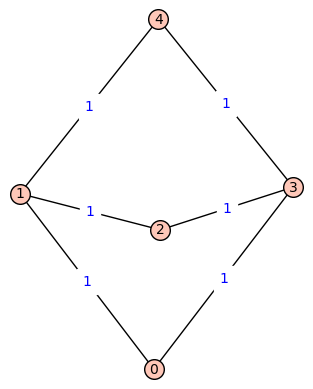
\includegraphics[scale=0.8]{prisme.png}
\caption{Graphe du prisme}
\label{prisme}
\end{figure}

On prend comme exemple la forme du prisme.

$$\Delta =  \left[\begin{array}{rrrrr}
2 & -1 & 0 & -1 & 0 \\
-1 & 3 & -1 & 0 & -1 \\
0 & -1 & 2 & -1 & 0 \\
-1 & 0 & -1 & 3 & -1 \\
0 & -1 & 0 & -1 & 2
\end{array}\right]
$$


$$\Delta^q = \left[\begin{array}{rrrr}
3 & -1 & 0 & -1 \\
-1 & 2 & -1 & 0 \\
0 & -1 & 3 & -1 \\
-1 & 0 & -1 & 2
\end{array}\right]
$$

Exemple de stabilisation:
\begin{eqnarray}
(0\ 6\ 0\ 0) & \mapsto^2 & (1\ 4\ 1\ 0)\\
& \mapsto^2 & (2\ 2\ 2\ 0)\\
& \mapsto^2 & (3\ 0\ 3\ 0)\\
& \mapsto^1 & (0\ 1\ 3\ 1)\\
& \mapsto^3 & (0\ 2\ 0\ 2)\\
& \mapsto^2 & (1\ 0\ 1\ 2)\\
& \mapsto^4 & (2\ 0\ 2\ 0)
\end{eqnarray}
On a ici une avalanche de taille 6 où 2 grains tombent dans le puits à l'étape 3 et 4.

Il y a $\det \Delta^q = 12$ configurations:
$$\left(2\ 1\ 2\ 1\right), \left(2\ 1\ 2\ 0\right), \left(1\ 1\ 2\ 0\right), \left(2\ 0\ 1\ 1\right), \left(0\ 1\ 2\ 1\right), \left(2\ 1\ 0\ 1\right),$$ 
$$\left(1\ 0\ 2\ 1\right), \left(2\ 0\ 2\ 0\right), \left(2,1\ 1\ 0\right), \left(1\ 1\ 2\ 1\right), \left(2\ 0\ 2\ 1\right), \left(2\ 1\ 1\ 1\right)$$

L'élément neutre est $(2\ 0\ 2\ 0)$.
Structure du groupe: $(\recu{G_q}, \plus) \simeq  \mathbb{Z}/2\mathbb{Z} \times \mathbb{Z}/6\mathbb{Z}$.

Le poids minimal est $\poidsmin{G_q} = 4$.



\chapter{Cas des graphe cycliques}
\section{Présentation}
\begin{figure}[h]
\centering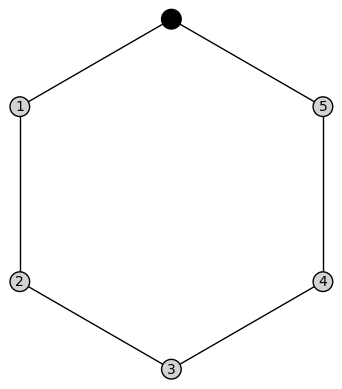
\includegraphics[scale=1]{6_cycle.png}
\caption{Graphe du 6-cycle, en noir le puits}
\label{6cycle}
\end{figure}
On va étudier une forme particulière de graphe : les cycles simples ($n+1$-cycle) que l'on note $C_{n+1}$.
Ces forme se révèlent très intéressantes car leur groupe est isomorphe à $\mathbb{Z}/(n+1)\mathbb{Z}$. On aura alors la propriété suivante:

\begin{property}[(2.6) \cite{thPoly}]
Tout groupe abélien fini est isomorphe au groupe d'un tas de sable.
\end{property}

\section{Configurations stable}

\begin{property}
L'ensemble des configurations stables positives est $\{0; 1\}^{n}$.
\end{property}
\begin{proof}
Tout les sommets ont exactement 2 arrêtes c'est-à-dire $\delta = (1\ 1\ \hdots \ 1)$. Donc les configurations stables ont moins de 1 grains sur chaque sommet.
\end{proof}

\section{Avalanches}

\begin{property}[Avalanche depuis un bord]\label{ava_bord}
$$(\hdots \ 0 \ 0\ 2\ [(1) * i]\ 0\ 0\ 0\ \hdots)$$ se stabilise en $$(\hdots \ 0 \ 1\ 1\ [(1) * (i - 1)]\ 0\ 1\ 0\ 0\ \hdots)$$
\end{property}
\begin{proof}
On démontre par récurrence qu'après $k \leq i$ éboulement on obtient la configuration: $$(\hdots \ 0 \ 1\ 1\ [(1) * (k-2)]\ 0\ 2\ [(1) * (i - k)]\ 0\ \hdots)$$
Initialisation:
On éboule l'unique case valant, deux et on obtient:
$$(\hdots \ 0 \ 1\ 0\ 2\ [(1) * (i - 1)]\ 0\ \hdots)$$
C'est à dire (avec la convention que [(1) * (-1)] enlève un 1):
$$(\hdots \ 0 \ 1\ 1\ [(1) * (-1)]\ 0\ 2\ [(1) * (i - 1))]\ 0\ \hdots)$$
Hérédité:
On suppose avoir fait $k$ éboulements, on a donc:
$$(\hdots \ 0 \ 1\ 1\ [(1) * (k-2)]\ 0\ 2\ [(1) * (i - k)]\ 0\ \hdots)$$
On éboule l'unique case valant, deux et on obtient:
$$(\hdots \ 0 \ 1\ 1\ [(1) * (k-2)]\ 1\ 0\ 2\ [(1) * (i - k - 1)]\ 0\ \hdots)$$
C'est à dire:
$$(\hdots \ 0 \ 1\ 1\ [(1) * (k+1-2)]\ 0\ 2\ [(1) * (i - (k+1))]\ 0\ \hdots)$$
Conclusion:
Après $i$ éboulements on arrive à:
$$(\hdots \ 0 \ 1\ 1\ [(1) * (i-2)]\ 0\ 2\ [(1) * (0)]\ 0\ \hdots)$$
C'est à dire:
$$(\hdots \ 0 \ 1\ 1\ [(1) * (i-2)]\ 0\ 2\ 0\ \hdots)$$
On éboule l'unique case valant, deux et on obtient le résultat annoncé:
$$(\hdots \ 0 \ 1\ 1\ [(1) * (i-2)]\ 1\ 0\ 1\ \hdots)$$
\end{proof}


\begin{theorem}[Avalanche depuis un centre]\label{ava_centre}
$$(\hdots \ 0 \ 0 \ [(1) * i]\ 2\ \ [(1) * j]\ 0\ 0 \hdots)$$ 
se stabilise en
$$(\hdots \ 0 \ [(1) * (j+1)]\ 0 \ [(1) * (i+1)]\ 0 \hdots)$$
\end{theorem}
\begin{proof}
On peut effectuer les éboulements dans un ordre quelconque. On effectue les stabilisations droite et par la proposition \ref{ava_bord} on a:
$$(\hdots \ 0 \ 0 \ [(1) * (i - 1)]\ 2\ 1 \ [(1) * (j - 1)]\ 0\ 1\ 0 \hdots)$$
C'est à dire:
$$(\hdots \ 0 \ 0 \ [(1) * (i - 1)]\ 2\ [(1) * (j)]\ 0\ 1\ 0 \hdots)$$
On démontre qu'après $k \leq i$ itérations du processus on a:
$$(\hdots \ 0 \ 0 \ [(1) * (i - k)]\ 2\ [(1) * (j)]\ 0\ [(1) * k]\ 0 \hdots)$$
Hérédité: on applique la proposition \ref{ava_bord} comme dans l'initialisation et on obtient:
$$(\hdots \ 0 \ 0 \ [(1) * (i - k - 1)]\ 2\ 1\ [(1) * (j - 1)]\ 0\ 1\ [(1) * k]\ 0 \hdots)$$
C'est à dire:
$$(\hdots \ 0 \ 0 \ [(1) * (i - (k+1))]\ 2\ [(1) * (j)]\ 0\ [(1) * (k+1)]\ 0 \hdots)$$
Conclusion:
après $i$ itérations on a:
$$(\hdots \ 0 \ 0 \ [(1) * (i - i)]\ 2\ [(1) * (j)]\ 0\ [(1) * i]\ 0 \hdots)$$
C'est à dire:
$$(\hdots \ 0 \ 0\ 2\ [(1) * (j)]\ 0\ [(1) * i]\ 0 \hdots)$$
On applique encore la proposition \ref{ava_bord} et on a:
$$(\hdots \ 0 \ 1\ 1\ [(1) * (j-1)]\ 0 \ 1\ [(1) * i]\ 0 \hdots)$$
C'est à dire:
$$(\hdots \ 0 \ [(1) * (j+1)]\ 0 \ [(1) * (i+1)]\ 0 \hdots)$$
\end{proof}


\begin{corollary}
Une avalanche causé par un grain est arrêté par un unique sommet à 0.
\end{corollary}


\section{Ordre du groupe}
\begin{property}[Ordre du groupe]
$\card{\recu{C_{n}}} = n$
\end{property}
\begin{proof}
On a $\card{\recu{C_n}} = \det\Delta^q$. On fait le calcul
en développant par rapport à la première colonne puis par rapport à la première ligne, on a:
\begin{eqnarray}
\card{\recu{C_n}} &=& \left|\begin{array}{rrrrrrr}
2 & -1 & 0 & 0 & \hdots & 0 & 0 \\
-1 & 2 & -1 & 0 & \hdots & 0 & 0 \\
0 & -1 & 2 & -1 & \ddots & \vdots & \vdots \\
0 & 0 & -1 & 2 & \ddots & 0 & 0 \\
\vdots & \ddots & \ddots & \ddots & \ddots & -1 & 0 \\
0 & 0 & \hdots & 0 & -1 & 2 & -1 \\
0 & 0 & \hdots & 0 & 0 & -1 & 2
\end{array}\right| \\
&=& 2 \card{\recu{C_{n-1}}} + 
\left|\begin{array}{rrrrrrr}
-1 & 0 & 0 & \hdots & 0 & 0 \\
-1 & 2 & -1 & \ddots & \vdots & \vdots \\
0 & -1 & 2 & \ddots & 0 & 0 \\
\vdots & \ddots & \ddots & \ddots & -1 & 0 \\
0 & \hdots & 0 & -1 & 2 & -1 \\
0 & \hdots & 0 & 0 & -1 & 2
\end{array}\right| \\
&=& 2 \card{\recu{C_{n-1}}} - \card{\recu{C_{n-2}}}
\end{eqnarray}
Or $\card{\recu{C_{0}}} = 0$ et $\card{\recu{C_{0}}} = 1$ donc en résolvant la relation de récurrence on a $\card{\recu{C_{n}}} = n$.
\end{proof}


\section{Configurations récurrentes}
\begin{theorem}[Description de \recu{C_{n+1}}]
$$\recu{C_{n+1}} = \delta \cup \bigcup_{i=1}^{n} \delta - e_i  $$
\end{theorem}
\begin{proof}
Une configuration stable $u$ qui n'est pas de la forme proposé est de la forme $$u = ([(1) * i] \ 0 \hdots \ 0 \ [(1) * j])$$. En effet, il y a au moins deux cases vides. En éboulant le puits on a alors $$u + \beta = (2\ [(1) * (i-1)] \ 0 \hdots \ 0 \ [(1) * (j-1)]\ 2)$$ Or par \ref{ava_bord} on sait que $$\stab{u + \beta} = (0\ [(1) * (i-2)] \ 0 \ 1 \hdots\ 1 \ 0 \ [(1) * (j-2)]\ 0) \not= u$$ donc d'après le critère de Dahr \ref{crit_dahr}, $u\not\in\recu{C_{n+1}} $.
\end{proof}
\begin{corollary} 
On retrouve $\card{\recu{C_{n+1}}} = n+1$.
\end{corollary}

\begin{corollary}\label{critere_cn}  $\poidsmin{C_{n+1}} = n - 1$
$$u \in \recu{C_{n+1}} \Leftrightarrow u \in \{0, 1\}^{n} \land \poids{u}\geq n - 1 $$
\end{corollary}
\begin{proof}
Il faut qu'il y ai exactement une ou zéro case vide et que des 1 ailleurs. D'où ce poids minimal.
\end{proof}

\section{Opérations}
\begin{theorem} \label{d+e}
$\delta_{n+1} \plus e_i = (\delta_{n+1} - e_{n+1-i})$
\end{theorem}

\begin{proof}
Cela découle du théorème \ref{ava_centre}. 
%\begin{huge}
%BOF
%\end{huge}
\end{proof}

\begin{theorem} \label{d-e+e}
$$(\delta_{n+1} - e_i) = ([(1) * (i - 1)\ 0\ [(1) * (n - 1 - i)])$$
Si $i < j$:
$$(\delta_{n+1} - e_i) \plus e_j = (\delta_{n+1} - e_{j-i})$$
Si $i = j$:
$$(\delta_{n+1} - e_i) \plus e_i = \delta_{n+1}$$
Si $i > j$:
$$(\delta_{n+1} - e_i) \plus e_j = (\delta_{n+1} - e_{n +j-i})$$
\end{theorem}

\begin{proof}
Cela découle du théorème \ref{ava_centre}. 
%\begin{huge}
%BOF
%\end{huge}
\end{proof}

\begin{property} \label{lemme1}
$\delta_{n+1} \plus e_i \plus e_{n+1-i} = \delta_{n+1}$
\end{property}
\begin{proof}
D'après \ref{d+e} : $\delta_{n+1} \plus e_i = \delta_{n+1} - e_{n+1-i}$. Et $\delta_{n+1} - e_{n+1-i} + e_{n+1-i} = \delta_{n+1}$.
\end{proof}

\begin{corollary} 
$\delta_{2n+1} \plus \delta_{2n+1} = \delta_{2n+1}$
\end{corollary}
\begin{proof}
On exprime $\delta_{2n+1} = \sum_{k=1}^{2n}e_k = \sum_{k=1}^{n}e_k + e_{2n+1-k}$. Or d'après la propriété \ref{lemme1}, ajouter $e_k$ et $e_{2n+1-k}$ ne change pas la configuration.
\end{proof}

\begin{corollary} 
$\delta_{2n} \plus \delta_{2n} = \delta_{2n} - e_n$
\end{corollary}
\begin{proof}
On exprime $\delta_{2n} = \sum_{k=1}^{2n}e_k = e_n + \sum_{k=1}^{n-1}e_k + e_{2n-k}$. Or d'après la propriété \ref{lemme1}, ajouter $e_k$ et $e_{2n-k}$ ne change pas la configuration. Donc $\delta_{2n} \plus{} \sum_{k=1}^{n-1}e_k + e_{2n-k} = \delta_{2n}$. On conclut avec \ref{d+e} que $\delta_{2n} \plus{} e_n = \delta_{2n+2} - e_n$
\end{proof}

\paragraph{Méthode de calcul}
$$(\delta_{2n+1} - e_i) \plus{} (\delta_{2n+1} - e_j)$$
Pour $i, j \leq n$ (sinon on change $k \not=i \land k \not=j$ par $2n+1-k \not=i \land 2n+1-k \not=j$):
\begin{eqnarray}
(\delta_{2n+1} - e_i) \plus{} (\delta_{2n+1} - e_j) 
&=& \delta_{2n+1} \plus{} \sum_{k=1; k \not=i \land k \not=j}^{2n} e_k\\
&=& \delta_{2n+1} \plus{} (e_{2n+1-i} + e_{2n+1-j} + \sum_{k=1; k \not=i \land k \not=j}^{n} e_k + e_{2n+1 - k})\\
&=& \delta_{2n+1} \plus{} e_{2n+1-i} \plus{} e_{2n+1-j}\\
&=& (\delta_{2n+1} - e_i) \plus{} e_{2n+1-j}
\end{eqnarray}
On peut alors finir le calcul avec \ref{d-e+e}.

$$(\delta_{2n} - e_i) \plus{} (\delta_{2n} - e_j)$$
Pour $i, j \leq n$ (sinon on change $k \not=i \land k \not=j$ par $2n+1-k \not=i \land 2n+1-k \not=j$):
\begin{eqnarray}
(\delta_{2n} - e_i) \plus{} (\delta_{2n} - e_j) 
&=& \delta_{2n} \plus{} \sum_{k=1; k \not=i \land k \not=j}^{2n-1} e_k\\
&=& \delta_{2n} \plus{} (e_{2n-i} + e_{2n-j} + e_n + \sum_{k=1; k \not=i \land k \not=j}^{n - 1} e_k + e_{2n - k})\\
&=& \delta_{2n} \plus{} e_n \plus{} e_{2n-i} \plus{} e_{2n-j}\\
&=& (\delta_{2n} - e_n) \plus{} e_{2n-i} \plus{} e_{2n-j}\\
&=& (\delta_{2n} - e_n) \plus{} e_{2n-i} \plus{} e_{2n-j}\\
\end{eqnarray}
On peut alors finir le calcul avec \ref{d-e+e}.



\begin{property}[Élément neutre pair]
L'élément neutre de \recu{C_{2n}} est $Id_{2n} = \delta_{2n} - e_n$.
\end{property}
\begin{proof}
Soit $u\in \recu{C_{2n}}$, $u = \delta_{2n} - e_i$ (on traite ici le cas $i \leq n$, on fait de même avec $i \geq n$):
\begin{eqnarray}
(\delta_{2n} - e_i) \plus{} (\delta_{2n} - e_n)
&=& \delta_{2n} \plus{} (e_{2n-i} + \sum_{k=1; k \not= i}^{n-1} e_k + e_{2n-k}) \\
&=& \delta \plus e_{2n-i} \\
&=& \delta_{2n} - e_i
\end{eqnarray}
\end{proof}

\begin{property}[Élément neutre impair]
L'élément neutre de \recu{C_{2n+1}} est $Id_{2n+1} = \delta_{2n+1}$.
\end{property}
\begin{proof}
Soit $u\in \recu{C_{2n+1}}$, $u = \delta_{2n+1} - e_i$ (on traite ici le cas $i \leq n$, on fait de même avec $i \geq n$):
\begin{eqnarray}
(\delta_{2n+1} - e_i) \plus{} \delta_{2n+1}
&=& \delta_{2n+1} \plus{} (e_{2n-i} + \sum_{k=1; k \not= i}^{n} e_k + e_{2n+1-k}) \\
&=& \delta \plus e_{2n+1-i} \\
&=& \delta_{2n+1} - e_i
\end{eqnarray}\end{proof}

\begin{property}[Itérés pairs]
$$ (\delta_{2n} - e_{n-1}) * k = (\delta_{2n} - e_{(n-1-k) \% (2n)})$$
\end{property}
\begin{proof}
Par récurrence.
\end{proof}

\begin{corollary}[Générateur pair] \label{gen_p}
$\omega(\delta_{2n} - e_{n-1}) = \omega(\delta_{2n} - e_{n+1}) = 2n $
\end{corollary}
\begin{proof}
On utilise la propriété précédente.
\end{proof}


\begin{property}[Itérés impairs]
$$ (\delta_{2n+1} - e_{n}) * 2k = (\delta_{2n+1} - e_{(n-k) \% (2n+1)})$$

$$ (\delta_{2n+1} - e_{n}) * (2k+1) = (\delta_{2n+1} - e_{(2n+1-k) \% (2n+1)})$$
\end{property}
\begin{proof}
Par récurrence.
\end{proof}

\begin{corollary}[Générateur impair] \label{gen_ip}
$\omega(\delta_{2n+1} - e_{n}) = \omega(\delta_{2n} - e_{n+1}) = 2n+1 $
\end{corollary}
\begin{proof}
On utilise la propriété précédente.
\end{proof}


\begin{theorem} \label{isocycle}
$(\recu{C_{n+1}}, \plus{}) \simeq \mathbb{Z}/(n+1)\mathbb{Z}$
\end{theorem}
\begin{proof}
$(\recu{C_{n+1}}, \plus{})$ est d'ordre $n+1$ et d'après \ref{gen_p} et \ref{gen_p} admet un générateur. C'est donc un groupe cyclique d'ordre $n+1$. Il est donc isomorphe à $\mathbb{Z}/(n+1)\mathbb{Z}$.
\end{proof}

\chapter{Multi-cycle}
\begin{figure}[h]
\begin{center}
\begin{subfigure}[b]{0.1\textwidth}
   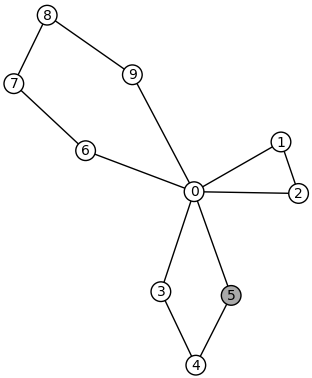
\includegraphics[width=3\linewidth, scale=2]{mcycle1.png}
   \caption{Graphe $C_3 \times C_4 \times C_5(5)$ , en gris le puits}
\end{subfigure} \hspace{6cm}%
\begin{subfigure}[b]{0.1\textwidth}
   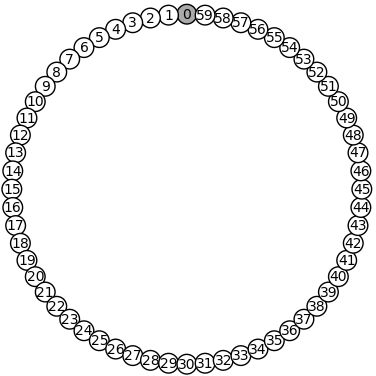
\includegraphics[width=3\linewidth, scale=2]{mcycle2.png}
   \caption{Graphe $C_60(0)$ , en gris le puits}
\end{subfigure}
\caption{Deux graphe dont les groupes sont isomorphes}
\end{center}
\end{figure}


On traite ici le cas de plusieurs cycle relier entre eux en 0. On note ainsi $C_{i_1} \times \hdots \times C_{i_n}(q)$ le produit de $n$ cycle de tailles $i_0, \hdots i_n$ avec le puits en $q$. On démontre alors le théorème suivant:
\begin{theorem} [Tas de sables chinois]
$(C_{i_1} \times \hdots \times C_{i_n}(q), \plus{}) \simeq (C_{\prod_{k=1}^{n} i_k}(0), \plus{}) \Leftrightarrow \forall k, k' \in \llbracket 1, n \rrbracket; i_k \land i_k' = 1$
\end{theorem}

\begin{proof}
D'après le théorème \ref{inv_puits}, on a $$(C_{i_1} \times \hdots \times C_{i_n}(q), \plus{}) \simeq (C_{i_1} \times \hdots \times C_{i_n}(0), \plus{})$$
On a donc plusieurs cycle qui n'interagissent pas car séparés par le puits. D'où: $$(C_{i_1} \times \hdots \times C_{i_n}(0), \plus{}) \simeq (C_{i_1}, \plus{}) \times \hdots \times (C_{i_n}(0), \plus{})$$
Or d'après le théorème \ref{isocycle}, on a:
$$(C_{i_1}, \plus{}) \times \hdots \times (C_{i_n}(0), \plus{}) \simeq \mathbb{Z}/(i_1)\mathbb{Z} \times \hdots \times \mathbb{Z}/(i_n)\mathbb{Z}$$
Or d'après le théorème des restes chinois:
$$\mathbb{Z}/(i_1)\mathbb{Z} \times \hdots \times \mathbb{Z}/(i_n)\mathbb{Z} \simeq \mathbb{Z}/ (\prod_{k=1}^{n} i_k)\mathbb{Z} \Leftrightarrow \forall k, k' \in \llbracket 1, n \rrbracket; i_k \land i_k' = 1$$
Or d'après le théorème \ref{isocycle}:
$$\mathbb{Z}/ (\prod_{k=1}^{n} i_k)\mathbb{Z} \simeq (C_{\prod_{k=1}^{n} i_k}, \plus{})$$
\end{proof}

\chapter{Géométrie}

On peut simuler des tas de sables sur des grilles triangulaires. On peut observer l'élément neutre et constater de fortes ressemblance avec la grille carré. On retrouve notamment un bande au milieu du neutre si la hauteur dépasse trop largement la longueur. L'existence de la bande pour une grille rectangulaire a déjà été prouvé. \cite{geoid}
\begin{conjecture}
Pour une grille triangle de $101 \times (94+2i)$ on observe i "deux- bandes".
\end{conjecture}

\begin{figure}[h]
\begin{center}
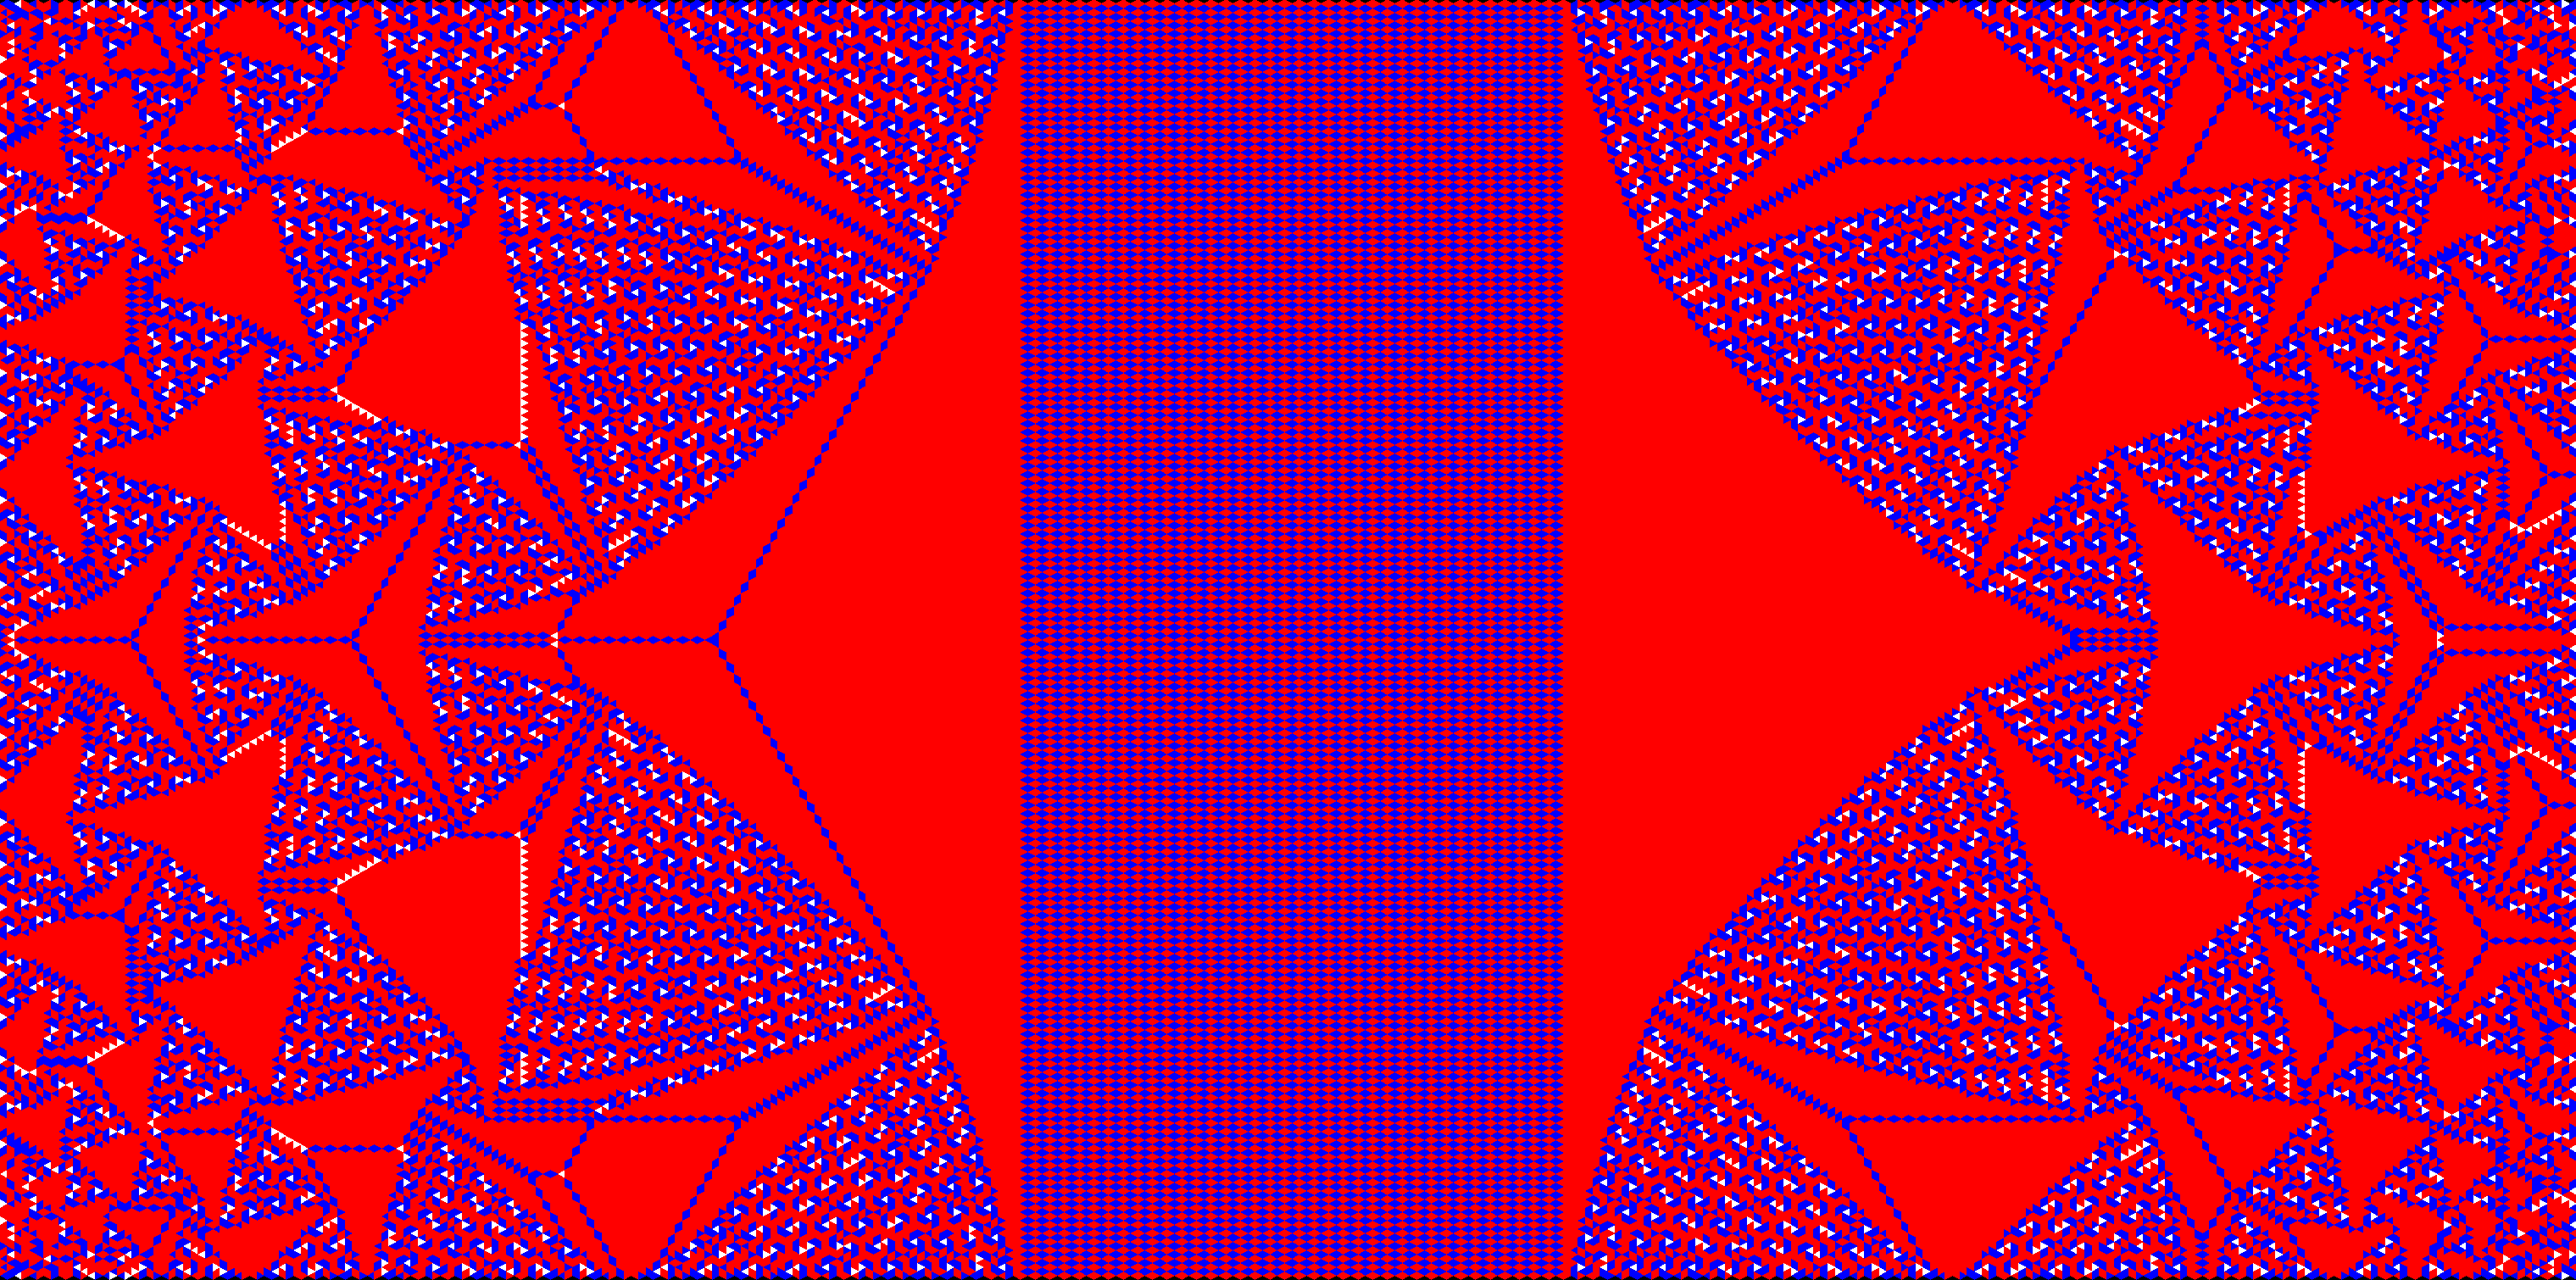
\includegraphics[scale=0.25]{351x301_e.png}
\caption{Element neutre sur un pavage triangulaire de 351x301}
\end{center}
\end{figure}


\bibliographystyle{plain}
\bibliography{tasAbelien}

\end{document}